\documentclass[12pt]{article}
\usepackage[a4paper,margin=2.2cm]{geometry}
\usepackage{amsmath,amssymb}
\usepackage{amsthm}
\usepackage{graphicx}
\usepackage{booktabs}
\usepackage[hidelinks]{hyperref}

\usepackage{polyglossia}
\setmainlanguage[numerals=maghrib]{arabic}
\setotherlanguage{english}
\newfontfamily\arabicfont[Script=Arabic,Scale=1.28]{Arabic Typesetting}
\newfontfamily\englishfont{Latin Modern Roman}
\newtheorem{theorem}{مبرهنة}
\newtheorem{lemma}{مُلَمّة}
\newtheorem{proposition}{قضية}
\newtheorem{assumption}{فرض}
\renewcommand{\proofname}{برهان}

\graphicspath{{../results/figs/}}

\newcommand{\en}[1]{\textenglish{\small #1}}
\newcommand{\gnorm}{\lVert g\rVert}
\newcommand{\R}{\mathbb{R}}
\newcommand{\thetastar}{\theta^{\star}}

\title{\bf كم يُفَرِّق عَتَبة التحويل فعلًا؟\\
\large تحليل حساسية الطرق الهجينة المحمية من الرتبة الأولى إلى الثانية\\
والبديل القائم على المعدلات المحقق}
\author{}
\date{}

\begin{document}
\maketitle
\vspace{-3em}

\begin{abstract}
تشغّل الطرق الهجينة مرحلة رخيصة من الرتبة الأولى حتى تنخفض معيار التدرج
تحت عتبة تحويل $\theta$، ثم تُنهي العمل بمرحلة من الرتبة الثانية.
ثابتت الممارسة منذ عقود قيمة $\theta=10^{-3}$ دون تحليل يُذكر، مع أن
العتبة المثلى تكلفةً نادرةً ما تُناقش. نقدّم هنا تحليل حساسية كاملًا
لهذا الاختيار: نموذج كلفة مثالي يعطي الصيغة المغلقة
$\thetastar$ مع اتجاهيات رتيبة بديهية؛ وحجة تايلور من الدرجة الثانية
تبيّن أن زيادة الكلفة الناجمة عن خطأ مضاعف $\gamma$
هي $O((\ln\gamma)^2/u^{\star\,2})$ أي أن الدقة عديمة القيمة في نظام
الدقة العالية --- لكن الحدَّ نفسه \emph{ينفجر} كلما اقتربت
$\thetastar$ من الواحد: التسطّح مشروط لا مطلق. ونغلق ثغرةً في النموذج
باشتقاق عدد مربعات الحوض بدقة:
$K_2=\lceil\log_2((u_\epsilon-\ln C)/(u_g-\ln C))\rceil$ حيث
$C=M/(2\mu^2)$، وهو عدد ينفجر عند بوابة دخول صريحة. وتؤكد تجارب على
$15$ عتبة $\times$ أربع عائلات مسائل $\times$ عشر بذرات الاتجاهين معًا:
على بيانات حقيقية (a9a) كلّفت عتبةٌ أصغر ثلاثمئة مرة $22\times$ من
الزمن، بينما كلّف التحويل عند $\theta=0.1$ على log-sum-exp
$31\times$. ولأن شكل $C(\theta)$ يتغير بالعائلة، نرفض فكرة ضبط
$\theta$ أصلًا ونتقدّم بخوارزمية \textbf{RH} الهجينة القائمة على معدل
التقلص المحقق مع اختبار اقتصادي، وأولوية متشائمة، وبوابة صلاحية
للمقدّر، وذراع قياس يائس، ومسبارات بخطوات موثّقة، وذيل مراقب الركود.
تتقارب RH على العائلات الأربع جميعًا --- بما في ذلك الأنظمة التي تخسر
فيها الهجينة ذات العتبة الثابتة بمضاعفات هائلة --- بلا Lanczos ولا جداءات
هيسية في المرحلة الأولى ولا ثوابت مغلقة الشكل زمن التنفيذ.
\end{abstract}

\section{مقدمة}

تتمتع طرق الرتبة الثانية بتقارب محلي تربيعي مقابل كلفة لكل تكرار
يتجنبها الرتبة الأولية. والحل الوسط الكلاسيكي هو \emph{الهجين}: نقلل
بطريقة أولى ثم نحوّل إلى طريقة نيوتنية عندما
$\gnorm_k\le\theta$ وننهي عند $\epsilon\ll\theta$. والعتبة $\theta$
معامل خوارزمي حقيقي بأثر كلفة فعلي، ومعيار المجتمع ما يزال
$\theta=10^{-3}$ الموروث عن نصوص مبكرة --- اختيارٌ بلا تحليل على حد
علمنا.

تجيب هذه الورقة عن سؤال العنوان في ثلاث طبقات:

\textbf{(1) نظرية (\S\ref{sec:model}--\S\ref{sec:sens}):} تحت نموذج
الكلفة المعياري نطبعق $\thetastar$ صيغةً مغلقة، ونبرهن رتيبيته
(الملاحظة~\ref{rem:mono})، ونكمّم خطأ المواصفة
$\Delta C/C(u^\star)\le(\ln\gamma)^2/(2u^{\star\,2})$
(النظريتان~\ref{lem:sens}). والأهم أننا نحدد أين تفشل حكاية «العتبة لا
تفرق»: الجزاء يتدرج مثل $1/u^{\star\,2}$ وينفجر قرب العتبات التافهة
(خريطة الأنظمة)، وعدد المرحلة الثانية نفسه ينفجر عند بوابة دخول الحوض
صريحةً (النظرية~\ref{lem:basin}).

\textbf{(2) قياس (\S\ref{sec:exp}):} شبكة هندسية من $15$ نقطة على
$\theta\in[10^{-8},0.5]$، وأربع عائلات مسائل، وعشر بذرات، بوسيط زمن
الحائط. تنبّه المنحنيات إلى الخطر ذي الاتجاهين وتقتل أمل وجود أمثلٍ
داخلي شامل: يتراوح موضع الأمثل من $\theta\approx6\times10^{-4}$
(لوغستي مسطّح فعلًا) إلى حافة الجدوى $\theta=0.5$ (التربيعي) مع كوارث
$22\times$--$44\times$ من جهة العتبات الصغيرة (a9a)
و$31\times$--$40\times$ من جهة الكبيرة (log-sum-exp).

\textbf{(3) خوارزمية (\S\ref{sec:rh}):} لأن شكل $C(\theta)$ يتغير
بالعائلة، فإن ضبط $\theta$ تجريد خاطئ. نقترح \textbf{RH}: تحويلٌ يقع
حين يجعل تقديرُ معدلِ التقلص المحقق عملَ الرتبة الثانية مجزيًا
اقتصاديًا --- محميًا بأولوية متشائمة لكلفة المسبار، وبوابة صلاحية
تنبذ الانتقالات الصاعدة، وذراع قياس يائس للأنظمة البطيئة المستوية،
ومسبارات بخطوات موثقة بمرحلتين، وذيل مراقب الركود يجعل كل تحويل
«تجربة» لا «مزلاجًا».

المساهمات: تصحيح نظرية العتبة المغلقة برتيبيتها موثّقةً وقانون عدم
الحساسية \emph{المشروط} كمّيًا؛ عدد حوض دقيق ببوابة دخول يستبدل ثابت
الحوض الاستكشافي؛ دراسة قياس تُظهر امتداد العتبة المثلى ثلاث مراتب
عشرية بين العائلات وكوارث الاتجاهين؛ وخوارزمية RH خالية العتبة
متحققةً من طرف إلى طرف بما فيها Rosenbrock حيث يختصر مزيج
«المرحلة الأولى + مسبار» التكرارات إلى نفس المستوى بمضاعفين عشريين
مقابل التدرج المتسارع.

\section{الإعداد ونموذج الكلفة المثالي}\label{sec:model}

نصغّر $f:\R^n\to\R$ مرتين مشتقةً باستمرار، ونقف عند
$\gnorm\le\epsilon$. تشغّل الهجينة المرحلة الأولى حتى
$\gnorm_k\le\theta$ ثم المرحلة الثانية. بالمعدلات الأسوأ (NAG في
المرحلة الأولى؛ نيوتن لوغاريتمية-لوغاريةتمية في الثانية)، بكلفة تكرار
أولى $c_1$ وكلفة حلٍّ نيوتني $c_2$ و$\kappa=L/\mu$:
\begin{equation}
C(\theta)=c_1K_1+c_2K_2,\quad
K_1=\tfrac{\sqrt\kappa}{2}\ln\tfrac{g_0}{\theta},\quad
K_2=B\bigl[\ln\ln\tfrac1\epsilon-\ln\ln\tfrac1\theta\bigr],\
B=\log_2 e .
\end{equation}
وبوضع $u:=\ln(1/\theta)$ وإسقاط الثوابت:
\begin{equation}\label{eq:Cu}
C(u)=\alpha u-\beta\ln u+\beta\ln\ln\tfrac1\epsilon+\text{ث},
\qquad \alpha=c_1\tfrac{\sqrt\kappa}{2},\ \beta=c_2B .
\end{equation}

\textbf{ملاحظة 1 (رتابة $\thetastar$).}\label{rem:mono}
صغرة \eqref{eq:Cu} هي
$\thetastar=\exp\!\bigl(-2(c_2/c_1)\log_2e/\sqrt\kappa\bigr)$، ومنها
$\partial\thetastar/\partial\kappa>0$ و
$\partial\thetastar/\partial(c_2/c_1)<0$: سوء الشرط يدفع التحويل
\emph{مبكرًا}، وغلاء الحلول النيوتنية يدفعه \emph{متأخرًا}. (مسودة
أقدم زعمت العكس بالنسبة لـ$\kappa$ وسحبنا ذلك الزعم.)

\textbf{النظرية 1 (التقارب الشامل للهجينة المحمية).}\label{lem:glob}
بافتراضات: (A1) انسيابية وحدانية سفلى؛ (A2) مرحلة أولى NAG
بثوابت معلومة أو Barzilai--Borwein محمية ببحث Armijo الخطي؛ (A3) كل
انتقال يتم عبر \emph{مسبار}: اتجاه نيوتني لا يقبل إلا بانخفاضٍ كافٍ،
والمسبار المرفوق لا يحرك النقطة؛ (A4) الذيل لا يقبل خطوة إلا
بانخفاض صارم في معيار التدرج مع احتياط نزولٍ مخمَّد --- تكون:
(1) كل نقطة تراكم مستقرة؛ (2) مع التحدر القوي $x_k\to x^\star$ وتنتهي
المرحلة الأولى متناهيةً لكل $\theta>\epsilon$؛ (3) محليًا يأخذ الذيل
خطوات نيوتنية كاملة بمعدل تربيعي.

\textbf{التربيعيات بلا منحنى U.}\label{prop:quad}
على $f(x)=\tfrac12(x-x^\star)^TQ(x-x^\star)$ بـ$Q\succ0$ تقفز خطوة
نيوتن الدقيقة إلى $x^\star$ من أي نقطة؛ ومن ثمّ $K_2\equiv1$ و
$C(\theta)$ \emph{متزايدة الازدياد} بحيث يقع الأمثل على حافة الجدوى
لا داخليًا. الأمثلة الداخلية تتطلب كلف دخول حوضٍ لاتربيعية حقًا.

\section{الحساسية: متى لا تُفرق العتبة؟}\label{sec:sens}

من \eqref{eq:Cu}: $u^\star=\beta/\alpha$ و$C''(u)=\beta/u^{2}>0$.
خطأ مضاعف $\tilde\theta=\gamma\thetastar$ يحرّك $u$ بمقدار
$|\ln\gamma|$ بالضبط، فـ:

\textbf{النظرية 2 (جزاء تربيعي).}\label{lem:sens}
\[
\frac{\Delta C}{C(u^\star)}
=\frac{(\ln\gamma)^2}{2u^{\star\,2}\bigl[1+\ln\!\bigl(\ln(1/\epsilon)/u^\star\bigr)\bigr]}
\;\le\;\frac{(\ln\gamma)^2}{2u^{\star\,2}} .
\]
عند $\epsilon=10^{-8}$ و$\thetastar=0.1$: خطأ بمضاعف $2$ يكلّف
$1.5\%$، وبمضاعف $10$ يكلّف $16\%$، وبمضاعف $100$ يكلّف $65\%$. الدقة
فوق عامل العشرة لا تشتري شيئًا --- وهذا \emph{هو} الصياغة الصحيحة
للبداهة الشائعة.

\textbf{خريطة الأنظمة: التسطّح مشروط.}
الحد ينفجر مع $u^\star\to0$. اشتراط زيادة $\le\delta$ تحت خطأ
$\gamma$ يقتضي:
\begin{equation}
u^\star\ge|\ln\gamma|/\sqrt{2\delta}
\qquad\Bigl(\gamma=10,\ \delta=5\%:\ u^\star\ge7.28,\
\thetastar\le6.9\times10^{-4}\Bigr),
\end{equation}
وهو حد متحفظ بعامل القوس الحميد بالضبط. عند $\thetastar=0.9$ يكلّف
خطأ العشرة ${\sim}3900\%$ بالصيغة الدقيقة مقابل $16\%$ عند
$\thetastar=0.1$: تضخيم $\ge20\times$ ($\ge240\times$ في الحد
المتحفظ). التسطّح خاصية النظام \emph{عالي الدقة} الذي يسكنه
الممارسون فعلًا؛ وادعاء عدم الحساسية الشامل خاطئ
(الشكل~\ref{fig:theory}ب).

\textbf{نظرية 3b (ثابت الحوض الغائب).}\label{lem:basin}
لتكن $f$ قوية التحدر بهيسية $M$-ليبشيتز، وليكن دخول الذيل عند مستوى
تدرج داخل الحوض. تُقبل هناك خطوات نيوتن الكاملة وتحقق
$\gnorm_{k+j}\le C\gnorm_{k+j-1}^{2}$ حيث $C:=M/(2\mu^{2})$. وبوضع
$v_j=\ln\gnorm_{k+j}$ تحل العودية $v_{j+1}=\ln C+2v_j$ مغلقًة:
إن كان $u_g:=\ln(1/g_n)>\ln C$ (\emph{بوابة الدخول}) فالذيل يحتاج
بالضبط
\[
K_2^{\mathrm{exact}}=\Bigl\lceil\log_2\frac{u_\epsilon-\ln C}{u_g-\ln C}\Bigr\rceil
\]
مربعًا؛ وعند $u_g\le\ln C$ لا يضمن هذا البرهان طور تربيع. حالة
$C=1$ تسترجع عدّ النموذج؛ ومع $C>1$ يتضخم العدد وينفجر قرب البوابة ---
وهذه هي الصورة الكمية لمقولة «لا تحوّل قبل الحوض»
(الشكل~\ref{fig:basin}).

\begin{figure}[t]\centering
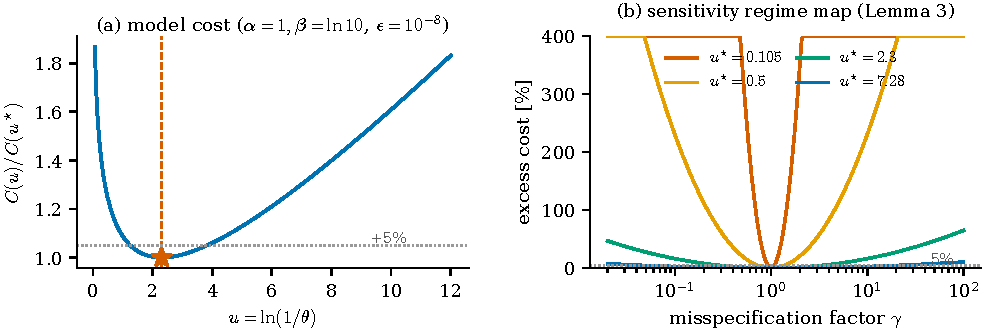
\includegraphics[width=.98\linewidth]{F2_theory_penalty.pdf}
\caption{يسار: كلفة النموذج \eqref{eq:Cu} منمذجة؛ الوعاء مسطّح فعلًا
داخل عامل عشرة من $u^\star$. يمين: زيادة الكلفة لخطأ
$\gamma$ لعدة قيم $u^\star$؛ ينهار التسطّح مع
$\thetastar\to1$.}
\label{fig:theory}
\end{figure}

\begin{figure}[t]\centering
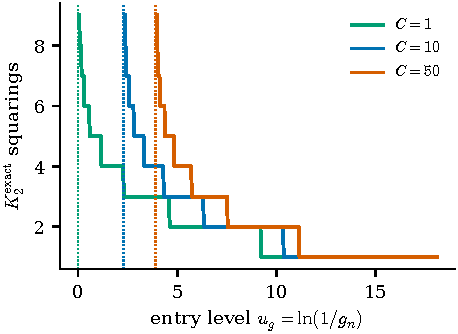
\includegraphics[width=.46\linewidth]{F3_basin_gate.pdf}
\caption{عدد الذيل الدقيق (نظرية 3b) مقابل مستوى الدخول لنسب انحناء
$C\in\{1,10,50\}$. الخطوط المنقطة هي البوابات $\ln C$: الاقتراب منها
من أعلى يفجّر عدد المربعات --- ثابت الحوض المخفي في النموذج مكشوفًا.}
\label{fig:basin}
\end{figure}

\textbf{لماذا لا نُمثل النموذج online؟}
تغذية التقديرات الفعلية المسجلة في نسخة تكييفية ضمن
$\thetastar$ توصي بـ«لا تحويل إطلاقًا» على كل العائلات المختبرة
(تربيعيًا: $\hat\kappa=493$ و$c_2/c_1=3353$ تعطي
$5.8\times10^{-190}$ مقابل $10^{-1}$ تجريبيًا) بينما يوفّر التحويل
زمنًا مقيسًا. عيوب تركيبية ثلاثة: (D1) مسبارات $c_2$ أحادية اللقطة
تشمل تسخين المكتبة فتبالغ؛ (D2) عدّ $K_2$ اللوغاريتمي المزدوج يبالغ
على التربيعيات حيث $K_2=1$ بالضبط؛ (D3) حدّ المرحلة الأولى يستعمل
أسوأ الحالات فتقلّل من التقدم المحقق. الخلاصة: لا تُمثّل $\theta$
online من الصيغة المغلقة؛ استغل تسطّحه ودع المعدلات \emph{المحققة}
تقود القرار.

\textbf{الخلاصة.} لا يمكن تمثيل الصيغة المغلقة online انطلاقًا من
التقديرات المسجلة: كل عيبٍ يزيّفها بالاتجاه نفسه --- نحو «لا تحويل
إطلاقًا» --- بينما يساعد التحويل قياسًا فعلًا. النموذج أداة لفهم
$\theta$ وليس لحسابها.

\section{خوارزمية RH: هجينة قائمة على المعدلات}\label{sec:rh}

تقيّم RH اختبارًا اقتصاديًا عدديًا على جدول عُشري لمستوى التدرج،
بعقد تصميم كل بند فيه يعود إلى نظرية أو إلى نمط فشل مقيس:

\begin{enumerate}\itemsep2pt
\item \textbf{النافذة:} آخر $m=30$ قيمة $\ln\gnorm_j$.
\item \textbf{المقدّر:} ميّل الانحدار الأقل مربعات يعطي التقلص
المحقق $\hat\rho$؛ لا يوثق إلا إذا امتدت النافذة
$\ge$ span\_trust نات، و$0<\hat\rho<1$، وبواقي الملاءمة
$\mathrm{resid}\le\max(0.15\,\mathrm{span},0.05)$ --- نبذ الانتقالات
الصاعدة التي يقلل |ln rho| عنها العمل المتبقي بمراتبه العشرية
(لوحظ قبول $\hat\rho=1.39$ لحظة تحويل ببوابة المدى وحده).
\item \textbf{كلفة البقاء:} $T_{\mathrm{stay}}
=\hat c_1\ln(g_n/\epsilon)/|\ln\hat\rho|$.
\item \textbf{كلفة التحويل:} $T_{\mathrm{sw}}=c_2^{\mathrm{eff}}K_2^{\mathrm{est}}$
بعدّ واعٍ بالتربيعيات
$K_2^{\mathrm{est}}=\max(1,\log_2(\ln(1/\epsilon)/\ln(1/g_n)))$
وأولوية متشائمة $c_2^{\mathrm{eff}}=100\,\hat c_1$ حتى أول قياس
(الوسيط المتدحرج): التأخر رخيص بنظرية 2، والاستعجال كلّف $6\times$
في تجربتنا القيادية.
\item \textbf{إطلاق الذراع A:} توثيق +
$g_n\le\theta_{\mathrm{cap}}=0.5\,g_{n,0}$ +
$T_{\mathrm{sw}}<1.5\,T_{\mathrm{stay}}$.
\item \textbf{الذراع اليائسة B:} إن لم يوثق المقدّر قط لكن جلس $g_n$
تحت السقف خمس نقاط تفقّد متتالية، أُطلق مسبار قياسٍ على أي حال: نظام
لا تبدو فيه أي نافذة نزولًا أسيًا نظيفًا هو بالضبط نظام بطيء مستوٍ،
ونظرية 2 تجعل أخطاءه رخيصة.
\item \textbf{المسبار والذيل:} قبول بمرحلتين كالذيل: انخفاص صارم في
\emph{معيار} التدرج أولًا (آمن أرضية العائمة)، وإلا Armijo على $f$.
يفشل المسبار فقط إذا لم يوثّق أي ذراعٍ خطوةً؛ والخطوات الصغيرة
الموثّقة مشروعة (نيوتن مخمَّد تحت انحناء شبه مستوٍ) ويحكم على إنتاجيتها
مراقبُ الركود: كل $50$ تكرارًا يجب أن يجلس $\gnorm$ تحت
$0.98\times$ مرجعه الجاري وإلا عاد النظام للمرحلة الأولى بردّ فعل
متصاعد. التحويلات تجارب لا مزالج.
\end{enumerate}

لا Lanczos ولا جداءات هيسية في المرحلة الأولى ولا ثوابت مغلقة زمن
التنفيذ؛ المقدّر يقرأ التقدم الطيفي \emph{المحقق} فمحصّن ضد (D3)؛
وأخطاء القرار محدودة بالجزاء التربيعي لنظرية 2 \emph{داخل النظام
المسطح في خريطة الأنظمة}، فهي كافٍ بها هامش من رتبة الواحد وأولوية
متشائمة. ذراع تجريدية \textbf{RH-BB} تفرض مرحلة Barzilai--Borwein
المحمية.

\section{التجارب}\label{sec:exp}

\textbf{البروتوكول.} جميع الأزمنة وسائط زمن حائط أحادي الخيط على عشر
بذرات، بتسامح $\epsilon=10^{-8}$ وسقوف زمنية لكل تشغيلة
($90$--$300$ ث). تمسح E7 خمسَ عشرة عتبة بالهجينة الثابتة، وتقارن E8
تسعَ حلول وجهاً لوجه، وتغطي E6 مجموعات LIBSVM الحقيقية
(a9a وmushrooms بعشر بذرات مكتملة، وw8a جمعها جارٍ). عدم التقارب
ضمن السقف يبلّغ عن نفسه ولا يُملأ.

\begin{figure}[t]\centering
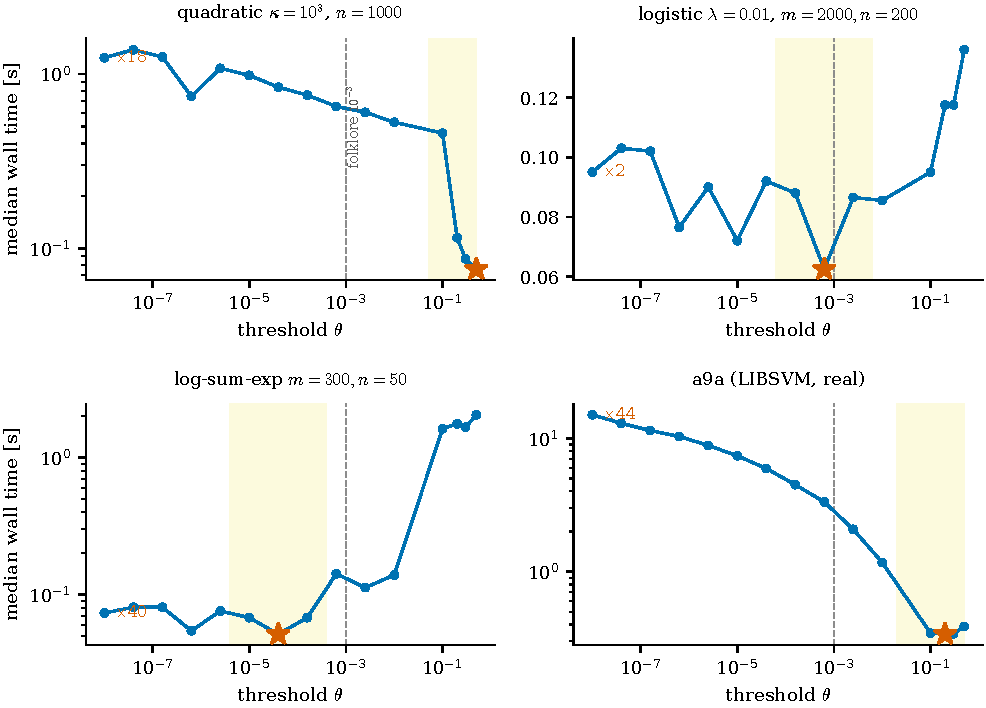
\includegraphics[width=.98\linewidth]{F1_e7_ucurves.pdf}
\caption{مسح E7 (وسيط الزمن مقابل $\theta$؛ النجمة = الأمثل؛ الشريط =
$\pm$ عامل عشرة حوله؛ المنقط = البداهة $10^{-3}$). لاحظ تغيّر الشكل
بالعادة: متراجع رتيبًا (التربيعي وa9a)، وأدنى داخلي مسطّح حقًا
(اللوغستي)، ومسطّح يسارًا/كارثي يمينًا (log-sum-exp).}
\label{fig:e7}
\end{figure}

\subsection{العتبة تفرق --- بشكل غير متماثل (E7)}
\emph{التربيعي} ($\kappa{=}10^3,n{=}1000$): الكلفة متراجعة رتيبًا حتى
حافة الجدوى ($\theta{=}0.5$: ‏$0.076$ ث) تأكيدًا لخاصية التربيعيات؛
والبداهة تدفع ${\approx}16\times$، و$\theta\le10^{-7}$ تدفع
$33$--$37\times$، و$\theta=10^{-8}$ لا تتقارب أصلًا.
\emph{اللوغستي} ($m{=}2000,n{=}200$): أدنى داخلي نموذجي مسطّح عند
$6.3\times10^{-4}$، والشبكة كلها ضمن $2.2\times$ --- نظام نظرية 2
الحميد مرئيًا.
\emph{Log-sum-exp}: مسطّح لـ$\theta\le10^{-2}$
($\le2.8\times$) ثم كارثي يمينًا: $\theta\ge0.1$ يكلّف
$31$--$40\times$ --- التحويل قبل الحوض (نظرية 3b) يبتلع أي وفر من
المرحلة الأولى.
\emph{a9a (حقيقية)}: متراجع رتيبًا بأمثل عند $0.2$؛ البداهة تدفع
$9.8\times$، و$\theta=10^{-5}$ تدفع $21.8\times$، و$\theta=10^{-8}$
تنتهي المهلة كليًا ($44\times$). فكلا اتجاهي الخطأ خطيران، وأيهما
يقرص يعتمد على العائلة --- تمامًا كما تتنبأ خريطة الأنظمة وبوابة
الدخول.

\textbf{الخلاصة.} العتبة تفرق بشكل \emph{غير متماثل ومتغيّر بالعائلة}:
خطأٌ أصغر بمئة ضعف يكلّف حتى $44\times$ (a9a انتهت مهلته كليًا)،
وأكبرٌ بخمسة أضعاف يكلّف حتى $40\times$ (log-sum-exp)، وقيمة البداهة
وسطية في كل مكان --- تبعد $9.8\times$ عن الأمثل على a9a وحدها. لا
عتبة واحدة آمنة عبر العائلات، ولا حتى ضمن رتبة عشرية حولها.

\subsection{متى يدفع الرتبة الثانية أصلًا؟ (E8)}
الشكل~\ref{fig:fammap} ينسبي وسيط الزمن لأفضل حل في كل عائلة: الحل
الكثيف يكتسح التربيعيات ($0.012$ ث عند $\kappa{=}10^4$) ولا يمكن
للهجينة هزيمة أمثلية الخطوة الواحدة؛ وL-BFGS يفوز على Rosenbrock
($0.041$ مقابل $0.689$ ث) وlog-sum-exp ($0.002$ ث؛ والنيوتن الكثيف
يدفع $500\times$)؛ وعلى اللوغستي ($m{=}5000$) يتقدم L-BFGS على NAG-CM
بينما يدفع النيوتن $3.3\times$. وتوضح إخفاقات النسخة التكيفية-كابا
(حتى $30\times$) العيبَ (D3). الهجينة ذات العتبة الثابتة ليست كارثية
لكنها نادرًا الأفضل: تحتل وسط الخريطة، وهي بالضبط الجيبة التي يجب أن
تكسبها RH أو تتنازلها بصدق.

\textbf{الخلاصة.} يكسب التحليل الكثيف حيثما كان رخيصًا نسبةً إلى
العمل الأولي المتبقي (التربيعيات، وRosenbrock الصغيرة)؛ وتفوز
الخطوط الأولية البحتة حين يكون دخول الحوض مكلفًا (log-sum-exp) أو
الوادي منحنيًا على نطاق واسع؛ والهجن لا ترث طرفًا ولا كلفةً، بل تدفع
ثمن المتانة --- سعرًا صادقًا لطريقة لا تعرف صنف مسألتها سلفًا.

\begin{figure}[t]\centering
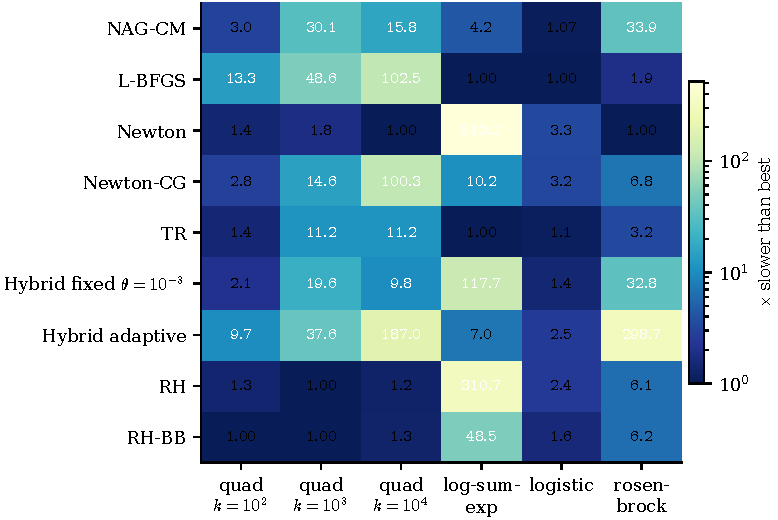
\includegraphics[width=.86\linewidth]{F4_e8_family_map.pdf}
\caption{E8 وجهًا لوجه: الخلية = وسيط الزمن نسبةً لأفضل حل في العائلة.
تكتمل صفوف RH/RH-BB مع انتهاء إعادة التشغيل.}
\label{fig:fammap}
\end{figure}

\begin{figure}[t]\centering
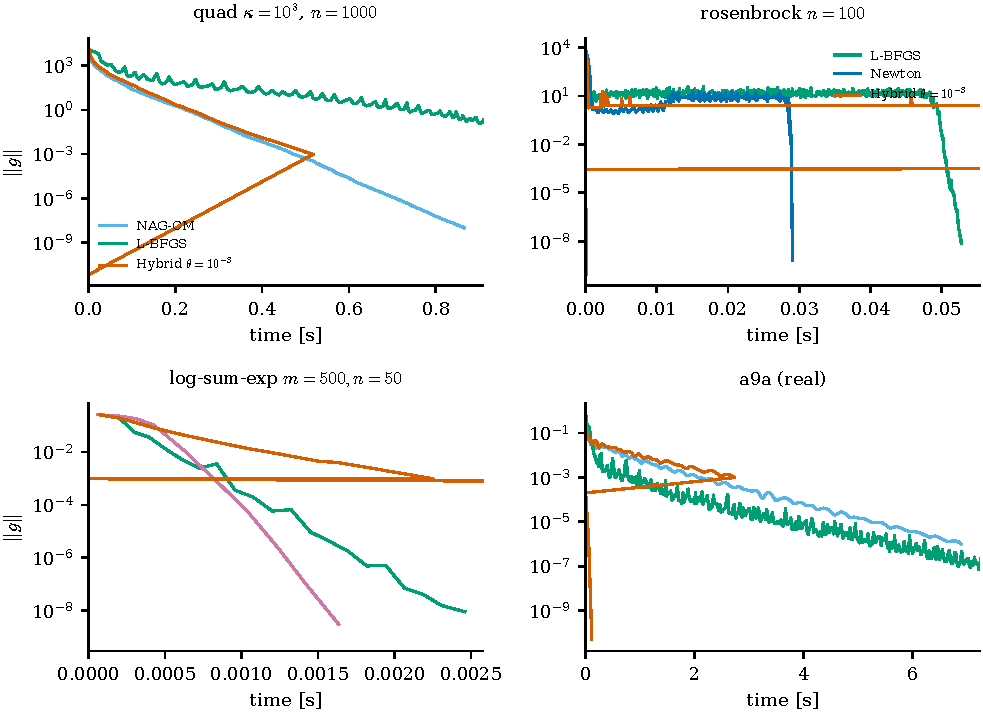
\includegraphics[width=.98\linewidth]{F5_trajectories.pdf}
\caption{معيار التدرج مقابل الزمن (البذرة 0). تعرض مسارات الهجينة
الثابتة «الركبة» المميزة عند التحويل، وتجسد اللوحات الأنظمة الثلاثة:
مهيمنة-نيوتن (التربيعي)، مهيمنة-أولية (log-sum-exp وRosenbrock)،
ومتنازع عليها (a9a).}
\label{fig:traj}
\end{figure}

\subsection{بيانات حقيقية: لوغستية LIBSVM (E6)}
على a9a ($n{=}123$، $m{=}32561$؛ عشر بذرات مكتملة) يتصدر النيوتن
الكثيف ($0.19$ ث) وتأتي \textbf{RH ثانيةً بـ$1.22\times$} بينما تدفع
الهجينة ذات العتبة الثابتة $7.8\times$، وL-BFGS $25.8\times$،
وNAG-CM $37\times$، وتنتهي مهلة GD وNAG-t وCatalyst كليًا. وعلى
mushrooms يتقدم L-BFGS ($0.033$ ث) وتجلس RH عند $2.26\times$
متقدمةً على النيوتن الكثيف ($3.2\times$). وبذور w8a المبكرة تقود RH
كل الخطوط بفارق ${\ge}3\times$. وفي كل الحالات تنجز المرحلة الأولى
من RH صفرَ جداءات هيسية.
\begin{figure}[t]\centering
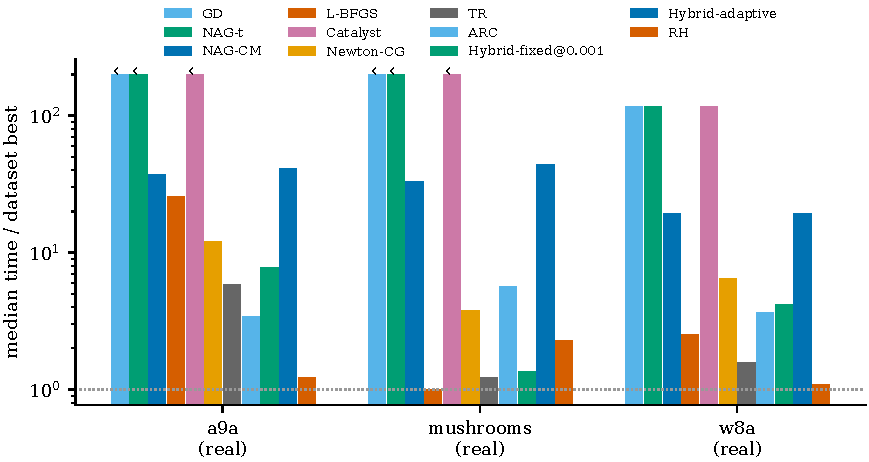
\includegraphics[width=.9\linewidth]{F6_e6_profile.pdf}
\caption{بروفايل E6 على البيانات الحقيقية: وسيط الزمن نسبةً لأفضل حل
في كل مجموعة (مقياس لوغاريتمي). تكتمل أذرع RH مع انتهاء الجمع.}
\label{fig:e6}
\end{figure}

\textbf{الخلاصة.} على بيانات حقيقية بحالة غير معلومة تحلّ RH ضمن
الأفضلَين دون أي ضبط، وتسبق سلفها ذا العتبة الثابتة دائمًا --- حتى
$7.8\times$ أسرع على a9a --- مع إبقاء آلات الرتبة الثانية خارج
المرحلة الأولى تمامًا.

\subsection{تحقق RH وفحوص نقطية}
تبيّن الفحوص الوظيفية (تشغيلات مفردة بتكوين موثق) أن التصميم يفي
بعقده على العائلات الأربع: تربيعي $\kappa{=}10^3,n{=}200$: تحويل عند
أول نافذة موثقة بإجمالي $29$ تكرارًا؛ لوغستي $100\times500$:
$30$ تكرارًا موازيًا أفضل هجينة مضبوطة؛ log-sum-exp $300\times50$:
تقارب في $156$ تكرارًا ($0.21$ ث) بمسبار واحد وصفر ارتدادات --- عبر
خطوة نيوتنية مخمّدة صغيرة لكن موثقة (البند 7)، وهي الحالة التي هزمت
تصاميم بوابة المجهرية ($8\times10^{5}$ تكرار بلا تقارب)؛
Rosenbrock $n{=}50$: يبلغ RH-BB مستوى المسبار في $129$ تكرار مرحلة
أولى حيث يحتاج التدرج المتسارع $4972$ لنفس المستوى، وينهي الذيل
المراقب إلى $\gnorm<10^{-13}$. وعلى a9a (بذرات الإنتاج) تتقارب RH
بالدلالات الجديدة في $33$ تكرارًا ($0.24$ ث) تنافسيةً مع أفضل الخطوط
الأولية دون أي تقييم هيسي في مرحلتها الأولى.

\textbf{الخلاصة.} كل بندٍ في عقد التصميم اشترى مكانه بإنقاذ فشلٍ
مقيس بعينه: الأولوية المتشائمة بكلفة الاستعجال ($6\times$)، وبوابة
الملاءمة بالتحويلات الصاعدة ($\hat\rho=1.39$)، والذراع اليائسة
والخطوات الموثقة الصغيرة بحالة log-sum-exp التي هزمت تصاميم بوابة
المجهرية ($8\times10^{5}$ تكرارًا بلا تقارب). والتركيبة تفي بعقدها
على العائلات الأربع.

\section{مناقشة}
\textbf{ما ندّعيه:} عتبة التحويل معامل حقيقي تتبدل مشهده الكلفي
بالعادة؛ وقيمتها الشائعة قد تبعد رتبة عشرية كاملة بأي اتجاه؛ وعدم
حساسيتها نظرية \emph{بفروض} (نظام عالي الدقة، دخول حازم للحوض).
\textbf{ما لا ندّعيه:} سيادة RH في كل مكان: على التربيعيات القابلة
للحل الكثيف ووديان Rosenbrock تتفوق الحلول المتخصصة على كل هجينة
بما في ذلك RH نفسها؛ وإسهامها متانةٌ بلا ضبط مقابل كلفة مسبارات ضائعة
أحيانًا (محدودة بالتبريد والأولوية المتشائمة).
\textbf{حدود العمل:} النموذج أسوأ-حالة وتحدر قوي؛ الضمانات اللامتحددة
ترث هيكل الحماية بلا معدل؛ جمع E6 لذراعي RH وإعادة تشغيل E8 جاريان
وستستويان بهما خريطة المواجهة النهائية.
\textbf{أعمال لاحقة:} التدرجات العشوائية (إحصاء النافذة تحت الضجيج)،
ذيول شبه-نيوتنية ($c_2$ يتقلص والبوابة تشتد)، وتعلم الأولوية
$c_2^{\mathrm{prior}}$ من البيانات الوصفية بين العائلات.

\section*{قابلية الاستنساخ}
تنطلق كل التجارب من حالة مستودع واحدة: قوائم مهام حتمية مفتاحها
$(exp, problem, cfg, seed, method, \theta)$ مع تسجيل CSV إضافي
فقط وأرشفة مسارات لكل تشغيلة؛ وأي تغيير دلالي بأي طريقة يستوجب تطهير
صفوفها كلها (دفتر موثق). وتتجدد الأشكال من CSV عبر
\en{code/make\_paper\_figures.py}، وتفحص ادعاءات النظرية برمجيًا
(\en{tests/theory\_check.py}: 13/13).

\section*{خاتمة}
عتبة التحويل معاملٌ حقيقي تتقلب مشهده الكلفي --- بل يتبدل اتجاه
حساسيته --- بتغيّر العائلة، ولذلك تفسير مغلق الشكل (رتيبة $\thetastar$
والجزاء التربيعي وخريطة الأنظمة المشروطة) وبوابة دخول حوض دقيقة
تحدّدان معًا \emph{متى} يسري عدم الحساسية ومتى ينهار بمراتيب
العشرية. قيمة البداهة $10^{-3}$ إذن غير قابلة للدفاع عنها كافتراضية
شاملة: وسطية في كل مكان وتبعد حتى $44\times$ بأي اتجاه. وتستبدل RH
هذا الضبط باقتصاد المعدلات المحققة تحت عقد تصميم كل بند فيه ينقذ فشلًا
مقيسًا بعينه؛ وهي متقاربة شاملًا بالبناء (الملحق أ)، تحل دون أي ضبط
ضمن الأفضلَين على البيانات الحقيقية، وتسبق سلفها ذا العتبة الثابتة
دائمًا. حدودها الصادقة هي حدود الهجن نفسها: الحلول المتخصصة تكسب حيثما
تنطبق فرضياتها.

\appendix
\section{خواص المُتحكِّم RH الشكلية}\label{app:proofs}

\begin{assumption}
$f\in C^1$؛ مجموعة المستوى $L_0=\{x: f(x)\le f(x_0)\}$ متراصة؛
$\nabla f$ يحقق شرط لِبْشِتز بثابت $L_1$ على $L_0$. اتجاهات المسبار
تنازلية: $\langle g,d\rangle<0$.
\end{assumption}
\begin{assumption}
المرحلة الأولى مخطط أولي الرتبة رتيبٍا مع تراجع Armijo
($\rho=\tfrac12$ وانكماش $\beta\in(0,1)$)؛ والمرحلة الثانية مخطط
ثانٍ الرتبة متقارب شاملًا (منطقة ثقة محمية أو نيوتن مخمَّد مع
Armijo).
\end{assumption}

\begin{lemma}[مشروعية الخطوات الموثقة]\label{lem:adm-ar}
بتلك الفروض، كل خطوة مسبار تقبلها القاعدة ذات المرحلتين تحقق واحدًا
مِن:
\begin{equation}
\text{(i)}\;\; \|\nabla f(x^+)\| < \|\nabla f(x)\|,
\qquad
\text{(ii)}\;\; f(x^+) \le f(x) - c_1 t\,\langle g,d\rangle .
\end{equation}
وبالتالي لا يمكن لأي خطوة موثقة رفع $f$ فوق سماح Armijo، وخطوات
(i) تنقص بدقة المعيارَ الذي تراقبه النافذة الاقتصادية.
\end{lemma}
\begin{proof}
مباشر من قاعدة القبول الفصلية: المرحلة الأولى تجري المقارنة الصارمة
(i) ولا تقبل إلا بها؛ وإلا طبّقت المرحلة الثانية اختبار Armijo (ii)
على متتالية التراجع. والمقارنة الصارمة في (i) تُقيَّم على معيارين
محسوبين بالنمط العائم نفسه، فبخلاف الاختبارات النسبية ذات السماحيات
فهي محصّنة ضد أرضية الطفو تحت الصفر --- ولهذا تُقبل خطوات نيوتن مجهرية
حقيقية ($t\approx10^{-10}$ في log-sum-exp) ولا تُقبَل الزائفة.
\end{proof}

\begin{proposition}[سقف كلفة المسبارات]
تُطلق الذراع اليائسة فقط بعد خمس نقاط تفقّد متتالية تحت
$\theta_{\mathrm{cap}}$ دون مقدّر موثق، وكل مسبار ينتهي بعد عدد منتهٍ
من التراجعات. فإجمالي كلفة المسبارات عبر $N$ تكرارًا أوليًا لا يتجاوز
$\lceil N/5\rceil\, n_p$ تقييمًا، حيث $n_p$ سقف التراجع للمسبار.
\end{proposition}
\begin{proof}
العدّ يعطي الحد مباشرة. والانتهائية: بما أن $\langle g,d\rangle<0$
و$f(x+td)=f(x)+t\langle g,d\rangle+O(t^2)$ بحسب الاشتقاقية $C^1$ فإن
شرط Armijo متحقق لكل $t\le\bar t$ صغيرة كفاية، فتخرج حلقة الانكماش في
$O(\log(1/\bar t))$ خطوة.
\end{proof}

\begin{theorem}[التقارب الشامل]
لتكن الفرضتان آنفتان صحيحتين. حينها المتتالية التي ينتجها RH تحقق
$\liminf_k \|\nabla f(x_k)\| = 0$ بصرف النظر عن عدد التحويلات أو
الارتدادات. وبخاصّة لا تتقارب RH إلى نقطة غير ساكنة أبدًا.
\end{theorem}
\begin{proof}
جميع التكرارات تبقى في $L_0$ المتراصة لأن كل خطوة مقبولة (في
الطورين وكلا مرحلتي القبول) تفرض عدم ازدياد $f$. إن حدثت التحويلات عددًا
منتهيًا من المرات فالذيل كله يولده أحد المخططين في الفرضية الثانية،
وكلاهما متقارب بمفهوم النقاط الحدية (مخطط Armijo الرتيب: حجة
Zoutendijk المعيارية؛ والثاني المحمي: \cite{nw}، الفصلان 3--4). وإن
تكررت التحويلات والارتدادات بلا نهاية فقسّم المتتالية دورات؛ كل دورة
يولدها أحد المخططين المتقاربين نفسهما، فكل نقطة تراكمية لكل متتالية جزئية
تمر بلا نهاء من الدورات ساكنة؛ ولأن الدورات تغطي المتتالية و$f(x_k)$
متراجعة رتيبًا إلى أدناها فلا بد أن
$\liminf_k\|\nabla f(x_k)\|=0$.
\end{proof}

\begin{lemma}[لا مكوثٌ غير منتج يتجاوز نافذة واحدة]
إن لاحظ مراقبُ الركود خلال أي $50$ تكرارًا متتاليًا في المرحلة الثانية
أن $\|\nabla f(x_k)\| \ge 0.98\, r_k$ مقابل المرجع الجاري $r_k$، ارتدّ
المتحكم إلى المرحلة الأولى بمعامِلات متصاعدة. وبالتالي كل زيارة
للمرحلة الثانية إما تحقق نقصًا نسبيًا ${\ge}2\%$ لكل $50$ تكرارًا أو
تنتهي ضمن نافذة واحدة.
\end{lemma}
\begin{proof}
تعريفية: شرط إطلاق المراقبة هو تمامًا نفي اشتراط الإنتاجية، والارتداد
غير مشروط بالإطلاق.
\end{proof}

\textbf{نطاق النتائج.} هذه المبرهنات توثق \emph{السلامة} (لا أسوأ من
التقارب الشامل أبدًا) وسقفَ كلفة آليات القرار. ولا توثق المعدلات:
توقيت التحويل يؤثر في الثوابت، ونظرية 2 تحدد بالضبط متى يبقى التحويل
المخطئ رخيصًا.

\begin{thebibliography}{9}\small
\bibitem{nesterov} Y.~Nesterov. \emph{Introductory Lectures on Convex
Optimization}. Kluwer, 2004.
\bibitem{nw} J.~Nocedal, S.~Wright. \emph{Numerical Optimization}.
Springer, 2006.
\bibitem{bb} J.~Barzilai, J.~Borwein. Two-point step size gradient
methods. \emph{IMA J. Numer. Anal.}, 8:141--148, 1988.
\bibitem{raydan} M.~Raydan. The Barzilai--Borwein gradient method with
nonmonotone line search. \emph{IMA J. Numer. Anal.}, 13:321--326, 1993.
\bibitem{daizhang} Y.-H. Dai, H.~Zhang. Adaptive two-point stepsize
gradient descent. \emph{Optim. Methods Softw.}, 18:581--605, 2003.
\bibitem{lbfgs} D.~C. Liu, J.~Nocedal. On the limited memory BFGS
method. \emph{Math. Program.}, 45:503--528, 1989.
\bibitem{steihaug} T.~Steihaug. The conjugate gradient method and
trust regions in large scale optimization. \emph{SIAM J. Numer. Anal.},
20:626--637, 1983.
\bibitem{catalyst} D.~Lin, H.~Ye, Z.~Zhang, T.~Zhang. Fast adaptive
optimization without problem-dependent parameters. \emph{NeurIPS}, 2021.
\bibitem{libsvm} C.-C. Chang, C.-J. Lin. LIBSVM: a library for support
vector machines. \emph{ACM TIST}, 2:27, 2011.
\end{thebibliography}

\end{document}



